\documentclass[UTF8]{article}
\usepackage{lmodern}
\usepackage{amssymb,amsmath}
\usepackage{ifxetex,ifluatex}
\usepackage{ctex}
\usepackage{fixltx2e} % provides \textsubscript
\ifnum 0\ifxetex 1\fi\ifluatex 1\fi=0 % if pdftex
  \usepackage[T1]{fontenc}
  \usepackage[utf8]{inputenc}
\else % if luatex or xelatex
  \ifxetex
    \usepackage{mathspec}
  \else
    \usepackage{fontspec}
  \fi
  \defaultfontfeatures{Ligatures=TeX,Scale=MatchLowercase}
\fi
% use upquote if available, for straig
ht quotes in verbatim environments
\IfFileExists{upquote.sty}{\usepackage{upquote}}{}
% use microtype if available
\IfFileExists{microtype.sty}{%
\usepackage[]{microtype}
\UseMicrotypeSet[protrusion]{basicmath} % disable protrusion for tt fonts
}{}
\PassOptionsToPackage{hyphens}{url} % url is loaded by hyperref
\usepackage[unicode=true]{hyperref}
\hypersetup{
            pdfborder={0 0 0},
            breaklinks=true}
\urlstyle{same}  % don't use monospace font for urls
\usepackage{longtable,booktabs}
% Fix footnotes in tables (requires footnote package)
\IfFileExists{footnote.sty}{\usepackage{footnote}\makesavenoteenv{long table}}{}
\usepackage{graphicx,grffile}
\makeatletter
\def\maxwidth{\ifdim\Gin@nat@width>\linewidth\linewidth\else\Gin@nat@width\fi}
\def\maxheight{\ifdim\Gin@nat@height>\textheight\textheight\else\Gin@nat@height\fi}
\makeatother
% Scale images if necessary, so that they will not overflow the page
% margins by default, and it is still possible to overwrite the defaults
% using explicit options in \includegraphics[width, height, ...]{}
\setkeys{Gin}{width=\maxwidth,height=\maxheight,keepaspectratio}
\IfFileExists{parskip.sty}{%
\usepackage{parskip}
}{% else
\setlength{\parindent}{0pt}
\setlength{\parskip}{6pt plus 2pt minus 1pt}
}
\setlength{\emergencystretch}{3em}  % prevent overfull lines
\providecommand{\tightlist}{%
  \setlength{\itemsep}{0pt}\setlength{\parskip}{0pt}}
\setcounter{secnumdepth}{0}
% Redefines (sub)paragraphs to behave more like sections
\ifx\paragraph\undefined\else
\let\oldparagraph\paragraph
\renewcommand{\paragraph}[1]{\oldparagraph{#1}\mbox{}}
\fi
\ifx\subparagraph\undefined\else
\let\oldsubparagraph\subparagraph
\renewcommand{\subparagraph}[1]{\oldsubparagraph{#1}\mbox{}}
\fi

% set default figure placement to htbp
\makeatletter
\def\fps@figure{htbp}
\makeatother


\date{}

\begin{document}

\section{Mathematical Statistics and Data Analysis}\label{header-n0}

\subsection{Joint Distributions}\label{header-n2}

\subsection{11810105 谢泽健}\label{header-n3}

\subsubsection{43.}\label{header-n4}

\(U_1\) 和 \(U_2\) 的分布均为

\[f_{U_{1}}(u)=f_{U_{2}}(u)=1, \quad u \in[0,1]\]

由卷积公式

\[f_{S}(s)=\int_{-\infty}^{\infty} f_{U_1}(u) f_{U_2}(s-u) \mathrm{d} u\]

当 \(0\le s\le1\)

\[f_{S}(s)=\int_{0}^{s} f_{U_1}(u) f_{U_2}(s-u) \mathrm{d} u=\int_{0}^{s} 1 \mathrm{d} u=s\]

当 \(0\le s\le1\)

\[f_{S}(s)=\int_{s-1}^{1} f_{U_1}(u) f_{U_2}(s-u) \mathrm{d} u=\int_{s-1}^{1} 1 \mathrm{d} u=2-s\]

综上

\[f_{S}(s)=\left\{\begin{array}{ll}{s} & {s \in[0,1]} \\ 
{2-s} & {s \in(1,2]}
\\ 0 & else
\end{array}\right.\]

\begin{figure}
\centering
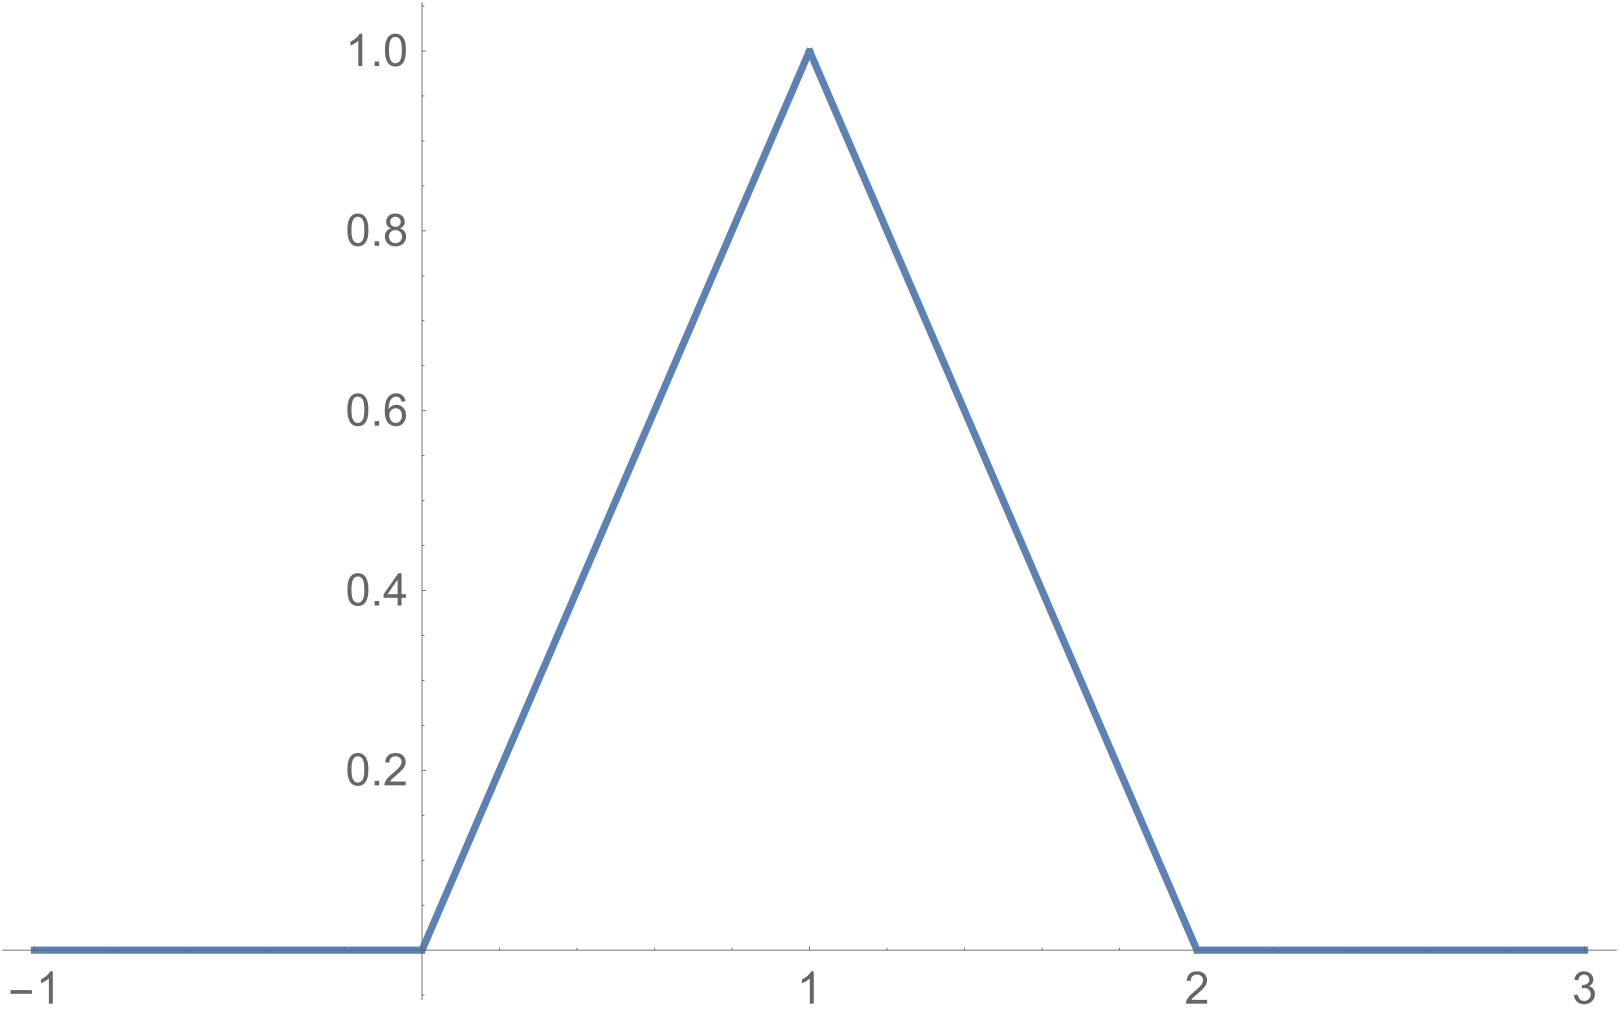
\includegraphics{C:/Users/g-odi/OneDrive/文档/SUSTech_ProbabilityTheory-and-Mathematical-Statistics_homework/assets/8-1.svg}
\caption{}
\end{figure}

\subsubsection{44.}\label{header-n16}

\(U_1\) 和 \(U_2\) 的分布均为

\[p_{U}(u)=\left\{\begin{array}{ll}
{\frac{1}{3}} & {u=0} \\ 
{\frac{1}{3}} & {u=1}\\
{\frac{1}{3}} & {u=2}
\end{array}\right.\]

由卷积公式

\[P\left(Z=z_{l}\right)=\sum_{i=1}^{\infty} P\left(X=x_{i}\right) P\left(Y=z_{l}-x_{i}\right)\]

当 \(0\le z\le2\)

\[p_{Z}(z)=\sum_{i=0}^{z} P\left(X=i\right) P\left(Y=z-i\right)=\sum_{i=0}^{z} \frac{1}{9} =\frac{z+1}{9}\]

当 \(2< z\le4\)

\[p_{Z}(z)=\sum_{i=z-2}^{2} P\left(X=i\right) P\left(Y=z-i\right)=\sum_{i=z-2}^{2} \frac{1}{9} =\frac{5-z}{9}\]

综上

\begin{longtable}[]{@{}llllll@{}}
\toprule
Z & 0 & 1 & 2 & 3 & 4\tabularnewline
\midrule
\endhead
P & \(\frac{1}{9}\) & \(\frac{2}{9}\) & \(\frac{3}{9}\) &
\(\frac{2}{9}\) & \(\frac{1}{9}\)\tabularnewline
\bottomrule
\end{longtable}

\subsubsection{51.}\label{header-n41}

令

\[\left\{\begin{array}{r}{x  y=z} \\ {y=y}\end{array}\right.\]

Jacobi式为

\[\frac{\partial(x, y)}{\partial(z, y)}=\left|\begin{array}{ll}{\frac{1}{y}} & {\frac{-z}{y^2}} \\ {0} & {1}\end{array}\right|=\left|\frac{1}{y}\right|\]

于是

\[F_{Z}(z)=\int_{-\infty}^{z}\left(\int_{-\infty}^{+\infty} f(\frac{u}{y}, y)\left|\frac{1}{y}\right| \mathbf{d} y\right) \mathbf{d} u\]

所以

\[f_{Z}(z)=\int_{-\infty}^{+\infty} f(\frac{z}{y}, y)|\left|\frac{1}{y}\right|| \mathbf{d} y\]

\subsubsection{52.}\label{header-n50}

令 \(X\) 和 \(Y\) 均为 均匀变量, 它们的联合分布为

\[f_{XY}(x,y)=1\]

令

\[\left\{\begin{array}{r}{\frac{x}{y}=z} \\ {y=y}\end{array}\right.\]

Jacobi式为

\[\frac{\partial(x, y)}{\partial(z, y)}=\left|\begin{array}{ll}{y} & {u} \\ {0} & {1}\end{array}\right|=\left|y\right|\]

于是

\[F_{Z}(z)=\int_{-\infty}^{z}\left(\int_{-\infty}^{+\infty} f(u y, y)\left|y\right| \mathbf{d} y\right) \mathbf{d} u\]

所以

当 \(z>1\)

\begin{aligned}
f_{Z}(z)=&\int_{-\infty}^{+\infty} f_{XY}(zy, y)\left|y\right| \mathbf{d} y
\\=&\int_{0}^{\frac{1}{z}} \left|y\right| \mathbf{d} y
\\=&\frac{1}{2z^2}
\end{aligned}

当 \(0\le z\le1\)

\begin{aligned}
f_{Z}(z)=&\int_{-\infty}^{+\infty} f_{XY}(zy, y)\left|y\right| \mathbf{d} y
\\=&\int_{0}^{1} \left|y\right| \mathbf{d} y
\\=&\frac{1}{2}
\end{aligned}

综上

\[f_{Z}(z)=\left\{\begin{array}{ll}{\frac{1}{2z^2}} & {z \in(1,\infty)} \\ 
\frac{1}{2} & {z \in[0,1]}
\\ 0 & else
\end{array}\right.\]

\subsubsection{57.}\label{header-n66}

\(Y_1\) 和 \(Y_2\) 的联合分布为

\[f_{Y_1Y_2}(y_1,y_2)=\frac{e^{-y_1^2+y_2 y_1-\frac{y_2^2}{2}}}{2 \pi }\]

用已知得

\[\left(
\begin{array}{cc}
 a_{11} & a_{12} \\
 a_{21} & a_{22} \\
\end{array}
\right).\left(
\begin{array}{c}
 y_1 \\
 y_2 \\
\end{array}
\right)=\left(
\begin{array}{c}
 x_1 \\
 x_2 \\
\end{array}
\right)\]

取矩阵的逆得到

\[\left(
\begin{array}{cc}
 \frac{a_{22}}{a_{11} a_{22}-a_{12} a_{21}} & -\frac{a_{12}}{a_{11} a_{22}-a_{12} a_{21}} \\
 -\frac{a_{21}}{a_{11} a_{22}-a_{12} a_{21}} & \frac{a_{11}}{a_{11} a_{22}-a_{12} a_{21}} \\
\end{array}
\right).\left(
\begin{array}{c}
 x_1 \\
 x_2 \\
\end{array}
\right)=\left(
\begin{array}{c}
 y_1 \\
 y_2 \\
\end{array}
\right)\]

Jacobi式为

\[\frac{\partial(y_1, y_2)}{\partial(x_1, x_2)}=\left|
\begin{array}{cc}
 \frac{a_{22}}{a_{11} a_{22}-a_{12} a_{21}} & -\frac{a_{12}}{a_{11} a_{22}-a_{12} a_{21}} \\
 -\frac{a_{21}}{a_{11} a_{22}-a_{12} a_{21}} & \frac{a_{11}}{a_{11} a_{22}-a_{12} a_{21}} \\
\end{array}
\right|=\left|\frac{1}{a_{11} a_{22}-a_{12} a_{21}}\right|\]

\(X_1\) 和 \(X_2\) 的联合分布为

\[f_{X_1X_2}(x_1,x_2)=\frac{\exp \left(-\frac{\left(a_{21}^2+2 a_{22} a_{21}+2 a_{22}^2\right) x_1^2+\left(-2 a_{11} a_{21}-2 a_{12} a_{21}-2 a_{11} a_{22}-4 a_{12} a_{22}\right) x_2 x_1+\left(a_{11}^2+2 a_{12} a_{11}+2 a_{12}^2\right) x_2^2}{2 \left(a_{12} a_{21}-a_{11} a_{22}\right){}^2}\right)}{2 \pi }\]

若 \(X_1\) 和 \(X_2\) 均为标准正态随机变量,

\[f_{X_1X_2}(x_1,x_2)=\frac{e^{\frac{1}{2} \left(-x^2-y^2\right)}}{2 \pi }\]

解得

\[\left(
\begin{array}{cc}
 a_{11} & a_{12} \\
 a_{21} & a_{22} \\
\end{array}
\right)=\left(
\begin{array}{cc}
 1 & 0 \\
 -1 & 1 \\
\end{array}
\right)\]

\subsubsection{70.}\label{header-n81}

\begin{aligned} F(x, y) &=\mathrm{P}\left(X_{n} \leqslant y\right)-\mathrm{P}\left(X_{1}>x, X_{n} \leqslant y\right) \\ &=[F(y)]^{n}-\mathrm{P}\left(x<X_{1} \leqslant y, x<X_{2} \leqslant y,\cdots, x<X_{n} \leqslant y\right) \\ &=[F(y)]^{n}-\prod_{i=1}^{k} \mathrm{P}\left(x<X_{i} \leqslant y\right) \\ &=[F(y)]^{n}-[F(y)-F(x)]^{k} \end{aligned}

\end{document}
